\section{Realizarea lucrarii de laborator:}

\begin{itemize}
	\item seteaza un branch to track a remote origin pe care vei putea sa faci push (ex. Github, Bitbucket or custom server)
	\\
	\\
	adaugam si selectam un nou branch pe nume "qwertMD"
	\begin{figure}[ht!]
		\centering
		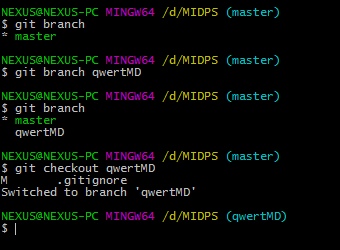
\includegraphics[width=90mm]{1.png}
	\end{figure}
	\\
	setam un branch to track remote origin si facem push
	\begin{figure}[ht!]
		\centering
		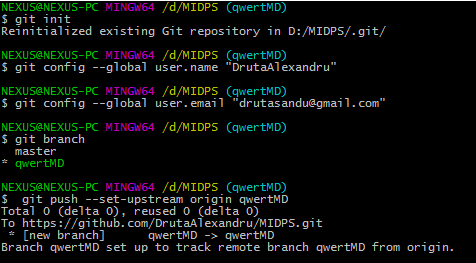
\includegraphics[width=90mm]{2.png}
	\end{figure}
	\\
	
	\item reseteaza un branch la commit-ul anterior
	\\
	\\
	verificam log-ul de commituri
	\begin{figure}[ht!]
		\centering
		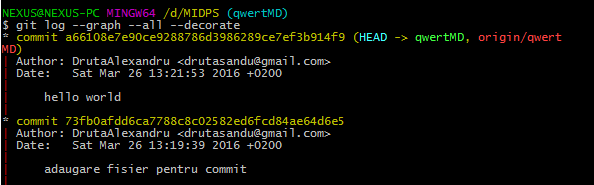
\includegraphics[width=90mm]{3.png}
	\end{figure}
	\\
	\\
	
	selectam din lista de commituri la un commit anterior prin introducerea inceputului codului de commit
	\begin{figure}[ht!]
		\centering
		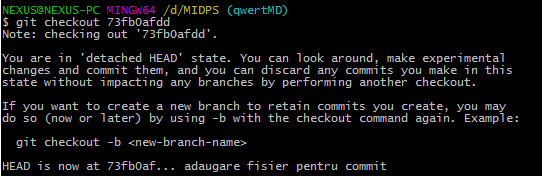
\includegraphics[width=90mm]{4.png}
	\end{figure}
	\\
	
	\item merge 2 branches
	\\
	\\
	facem merge la cele 2 branch-uri in unul singur master
	\begin{figure}[ht!]
		\centering
		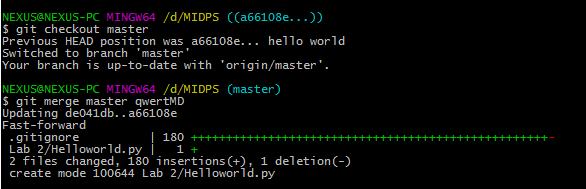
\includegraphics[width=90mm]{5.png}
	\end{figure}
	\\
	\\
	
	\item rezolvarea conflictelor a 2 branches
	\\
	\\
	executam comanda de merge
	\begin{figure}[ht!]
		\centering
		
\includegraphics[width=90mm]{6.png}
	\end{figure}
	\\
	\\
	
	observam ca a aparut o eroare in fisierul Helloworld.py, astfel git a modificat fisierul sa alegem singuri care cod sal lasam
	\begin{figure}[ht!]
		\centering
		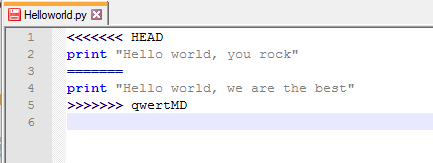
\includegraphics[width=90mm]{7.png}
	\end{figure}
	\\
	\\
	
	am schimbat fisierul selectind codul care ne trebuie
	\begin{figure}[ht!]
		\centering
		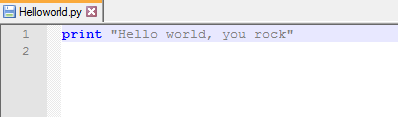
\includegraphics[width=90mm]{8.png}
	\end{figure}
	\\
	\\
	
	executam commit-ul de merge a celor 2 branch-urilor deja cu conflictul rezolvat
	\begin{figure}[ht!]
		\centering
		
\includegraphics[width=90mm]{9.png}
	\end{figure}
	\\
	\\
	
	\item Bonus point: Compilarea scripturilor HelloWorld projects 
	\\
	\\
	compilarea scriptului in java
	\begin{figure}[ht!]
		\centering
		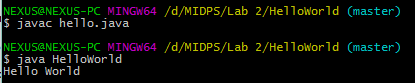
\includegraphics[width=90mm]{10.png}
	\end{figure}
	\\
	
	compilarea scriptului in python
	\begin{figure}[ht!]
		\centering
		
\includegraphics[width=90mm]{11.png}
	\end{figure}

\end{itemize}
